\documentclass[10pt,a4paper]{amsart}
\usepackage[margin=19mm]{geometry}
\usepackage{amsmath,amssymb,mathtools}
\usepackage[scr=rsfs,cal=euler]{mathalfa}
\usepackage{xfrac}
\usepackage[unicode,hidelinks,bookmarks=false]{hyperref}
\newcommand{\ie}{i.e.\ }
\newcommand{\cf}{cf.\ }
\newcommand{\resp}{respectively\ }
\newcommand{\Subsection}{\subsection}
\providecommand{\nobreakdash}{\nobreak\hbox{-}}
\setlength{\emergencystretch}{2em}
\multlinegap0pt
\usepackage{tikz}
\usepackage{amssymb}
\usepackage{mathtools}
\usepackage[shortlabels]{enumitem}
\usepackage{float}
\newtheorem{lma}{Lemma}
\newtheorem{prop}{Proposition}
\def\A{\ensuremath{\mathscr A}}
\def\F{\ensuremath{\mathcal F}}
\renewcommand{\i}{\mathtt{i}}
\renewcommand{\j}{\mathtt{j}}
\renewcommand{\k}{\mathtt{k}}
\def\sm{\setminus}
\title{Dynamical blanket times}
\author{Natalia Jurga, Mike Todd}
\date{Source: arXiv:2606.18926v1 (CC BY 4.0)}
\begin{document}
\maketitle

\noindent\emph{Source and licence.} Dynamical blanket times. Version arXiv:2606.18926v1 (CC BY 4.0), distributed by arXiv under the Creative Commons Attribution 4.0 International licence, http://creativecommons.org/licenses/by/4.0/, as recorded in the arXiv licence metadata for this exact version and shown on the abstract page https://arxiv.org/abs/2606.18926v1. Full licence notice: \texttt{licenses/arxiv-2606.18926-CC-BY-4.0.txt}.\par\smallskip

\noindent\textit{Editorial scope.} Counted unit: the article's prop mainmf (source0.tex lines 1005--1014). The article's complete original proof of it is delivered with it (source0.tex lines 1016--1100, one \texttt{proof} environment of 85 lines). No mathematics is written, repaired or re-derived: the statement and the proof are the article's own lines, in the article's own notation, and no retained line is substituted or re-flowed.  Retained uncounted as the source-local context the proof needs: lines 941--944.  Nothing was omitted from any retained span, so the package carries no omission record.  No retained line contains a citation, so the wrapper carries no bibliography and no bibliography entry.  The retained lines contain the article's own diagram code, which the wrapper typesets with the standard tikz packages; no image file is delivered and the package declares no asset dependency.  Editorial formatting only, in addition: an AMS \texttt{amsart} preamble that restates the article's own declarations and macros used by the retained lines, namely the environments \texttt{lma}, \texttt{prop} on separate counters, together with the standard packages those lines need.  The retained environments print in this document as Lma 1, Proposition 1 in order of appearance, whereas the article prints the same items with the numbering of its own full document.  The complete native source of the article as distributed in the arXiv e-print for this exact version is bundled unchanged as \texttt{sources/203105/source0.tex}.
\begin{lma}\label{mfacip}
$\mathcal{F}_\mu(D)=1$ if and only if $\mu$ is the absolutely continuous
invariant probability measure (acip) for $f$.
\end{lma}

\begin{prop}\label{mainmf} Let $\mu$ be any measure which is not an acip.  Letting  $\mathbf{C}_\delta= p\delta^{-D}\log(1/\delta)$ for an appropriate choice of $p$, the following holds. 
For all sufficiently small $\epsilon, \delta \in (0,1)$ and sufficiently small
$$0<r<\frac{d}{2}(1-\F_\mu(D))$$
we can construct an $(\epsilon,\delta)$-multifractal discretisation of $\mu$ such that  $\A_{\delta,\epsilon}=\A_{\delta,\epsilon}^1\cup \A_{\delta,\epsilon}^2$ and 
\begin{align*}
\sum_{A \in \A^1_{\delta,\epsilon}} e^{-\mathbf{C}_\delta \mu(A)}& \leq \epsilon^{-\frac{1}{d}}\delta^{-\frac{D}{d}}\delta^{\delta^{-r}/2}, \\
\sum_{A \in \A^2_{\delta,\epsilon}} e^{-\mathbf{C}_\delta \mu(A)} &\leq\epsilon^{-\frac{1}{d}} \delta^{\frac{1}{2}-\frac{r}{d}-\frac{\F_\mu(D)}{2}}.
\end{align*}
Moreover each $A \in\A_{\delta,\epsilon}$ is made up of a finite union of cylinders.
\end{prop}

\begin{proof}
By Lemma \ref{mfacip} we know that the multifractal spectrum $\F_\mu(D)<1$. First we describe how to construct $ \A^1_{\delta,\epsilon}$. For now, $r>0$ can be arbitrary. Let us denote 
$$\rho(\epsilon,\delta):=\epsilon^{\frac{1}{d}}\delta^{\frac{D}{d}}$$ and let $\mathscr{P}_{\rho(\epsilon,\delta)}$ denote the canonical partition. Let $\mathcal{B}_{\rho(\epsilon,\delta)}$ consist of all intervals $J$ which can be written as a union of cylinders from $\mathscr{P}_{\rho(\epsilon,\delta)}$ and which have length $|J| \in [2\delta-2\rho(\epsilon,\delta), 2\delta]$, i.e., 
$$\mathcal{B}_{\rho(\epsilon,\delta)}:= \left\{ J \text{ an interval}: J= C_1\cup\cdots \cup C_k \text{ and } C_i\in \mathscr{P}_{\rho(\epsilon,\delta)} \text{ for } i=1, \ldots, k\right\}.$$
 We define
$$\A^1_{\delta,\epsilon,r}:=\{J \in \mathcal{B}_{\rho(\epsilon,\delta)}: \mu(J) \geq \delta^{D-r}/2\}.$$
Then 
$$\#\A^1_{\delta,\epsilon,r} \lesssim \rho(\epsilon,\delta)^{-1}=\epsilon^{-\frac{1}{d}}\delta^{-\frac{D}{d}}$$
and for any $A \in \A^1_{\delta,\epsilon,r}$ we have $\mu(A)\delta^{-D} \geq \delta^{-r}/2$ therefore for $p \geq 1$,
$$\sum_{A \in \A^1_{\delta,\epsilon,r}} e^{-\mathbf{C}_\delta \mu(A)} \leq \epsilon^{-\frac{1}{d}}\delta^{-\frac{D}{d}}\delta^{\delta^{-r}/2}.$$
This demonstrates the first inequality in Proposition \ref{mainmf}, when we later define $\A^1_{\delta,\epsilon}$ by $\A^1_{\delta,\epsilon}=\A^1_{\delta,\epsilon,r}$ for an appropriate choice of $r>0$. 

Next, we describe how to construct $ \A^2_{\delta,\epsilon}$. Since $\F_\mu(D)<1$ we can fix 
$$0<r<d\left(\frac{1}{2}-\frac{\F_\mu(D)}{2}\right)$$
sufficiently small such that 
$$\#\mathscr{P}_{\delta/2}^r \leq \delta^{-\frac{1}{2}-\frac{\F_\mu(D)}{2}}$$
 where
$$\mathscr{P}_{\delta/2}^r:=\left\{C \in \mathscr{P}_{\delta/2}: \mu(C) < \delta^{D-r}\right\}$$
and $\mathscr{P}_{\delta/2}$ is the canonical partition. Note that since $\F_\mu(D)<1$, the exponent in the upper estimate on $\#\mathscr{P}_{\delta/2}^r$ satisfies the bounds $\F_\mu(D)< \frac{1}{2}+\frac{\F_\mu(D)}{2}<1.$


Consider an interval $U \in\mathscr{P}_{\delta/2} \setminus\mathscr{P}_{\delta/2}^r$ which neighbours an interval $V \in\mathscr{P}_{\delta/2}^r$. Let $\mathbf{k}$ be the shortest word for which $\Pi[\mathbf{k}] \subset U$, the interval $\Pi[\mathbf{k}]$  neighbours $V$ and  $\mu(\Pi[\mathbf{k}])<\delta^{D-r}$, see Figure \ref{fig:k} below. Let $\mathcal{Q}_\delta^r$ consist of all $\mathbf{k}\in \Sigma^*$ which can be obtained in this way for some $U \in\mathscr{P}_{\delta/2} \setminus\mathscr{P}_{\delta/2}^r$ and $V \in\mathscr{P}_{\delta/2}^r$. 

\begin{figure}[h]
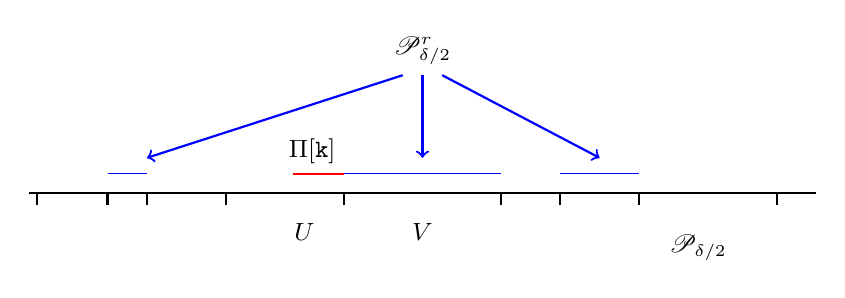
\begin{tikzpicture}[thick, scale=0.5]
\draw[ - ] (0,2) -- (20,2);
\draw[ - ] (2,1.7) -- (2, 2);
\draw[ - ] (3,1.7) -- (3, 2);
\draw[ - ] (5,1.7) -- (5, 2);
\draw[ - ] (8,1.7) -- (8, 2);
\draw[ - ] (12,1.7) -- (12, 2);
\draw[ - ] (13.5,1.7) -- (13.5, 2);
\draw[ - ] (15.5,1.7) -- (15.5, 2);
\draw[ - ] (19,1.7) -- (19, 2);
\draw[ - ] (0.2,1.7) -- (0.2, 2);

\draw[thin, blue, - ] (2,2.5) -- (3, 2.5);
\draw[ thin, blue, - ] (8,2.5) -- (12, 2.5);
\draw[thin,  blue, - ] (13.5,2.5) -- (15.5, 2.5);
\draw[thick, red, - ] (6.7,2.5) -- (8, 2.5);

\draw (7,1.5) node[below] {{\small $U$}};
\draw (10,1.5) node[below] {{\small $V$}};

\draw (7.2,2.5) node[above] {{\small $\Pi[\k]$}};

\draw (17,1.2) node[below] {{\small $\mathscr{P}_{\delta/2}$}};

\draw (10,5) node[above] {{\small $\mathscr{P}_{\delta/2}^r$}};

\draw[blue, ->] (9.5, 5)--(3, 2.9);

\draw[blue, ->] (10, 5)--(10, 2.9);

\draw[blue, ->] (10.5, 5)--(14.5, 2.9);
\end{tikzpicture}
  \caption{The long black line here is a segment of $[0, 1]$ and the main partition of this segment represents $\mathscr{P}_{\delta/2}$, and the thin blue intervals belong to $\mathscr{P}_{\delta/2}^r$. For the indicated neighbouring intervals $U\in \mathscr{P}_{\delta/2}\sm \mathscr{P}_{\delta/2}^r$ and $V\in \mathscr{P}_{\delta/2}^r$, the thick red interval $\Pi[\k]$ is chosen as the cylinder of shortest symbolic length contained in $U$, adjacent to $V$ and whose measure is at most $\delta^{D-r}$.}
    \label{fig:k}
\end{figure}

Define 
$$\kappa(\epsilon,\delta):=\epsilon^{\frac{1}{d}}\delta^{\frac{r}{d}}$$
and let $\mathscr{P}_{\kappa(\epsilon,\delta)}$ be the canonical partition.

Now define $\A^2_{\delta,\epsilon}$ to be all intervals $J$ which can be written as a union of cylinders from  
\begin{equation}\label{weirdset}
 \left\{\Pi[\i\j]: \Pi[\i] \in \mathscr{P}_{\delta/2}^r, \;\Pi[\j ]\in \mathscr{P}_{\kappa(\epsilon,\delta)}\right\} \cup \left\{\Pi[\k^-\j]: \mathbf{k} \in \mathcal{Q}_{\delta}^r,\; \Pi[\j] \in \mathscr{P}_{\kappa(\epsilon,\delta)}\right\}
\end{equation}
and which have length $|J| \in [2\delta-2\rho(\epsilon,\delta), 2\delta]$. Since $\#\mathscr{P}_{\delta/2}^r \leq\delta^{-\frac{1}{2}-\frac{\F_\mu(D)}{2}}$,
$$\#\A^2_{\delta,\epsilon} \lesssim\delta^{-\frac{1}{2}-\frac{\F_\mu(D)}{2}}\kappa(\epsilon,\delta)^{-1}=\epsilon^{-\frac{1}{d}} \delta^{-\frac{r}{d}-\frac{1}{2}-\frac{\F_\mu(D)}{2}}.$$
In particular, for $p\ge 1/a$, 
$$\sum_{A \in \A^2_{\delta,\epsilon}} e^{-\mathbf{C}_\delta \mu(A)} \leq\delta \cdot\epsilon^{-\frac{1}{d}} \delta^{-\frac{r}{d}-\frac{1}{2}-\frac{\F_\mu(D)}{2}}=\epsilon^{-\frac{1}{d}} \delta^{\frac{1}{2}-\frac{r}{d}-\frac{\F_\mu(D)}{2}}.$$

We define $\A^1_{\delta,\epsilon}=\A^1_{\delta,\epsilon,r}$ for the choice of $r$ which was fixed in the construction of $\A^2_{\delta,\epsilon}$ and set $\A_{\delta,\epsilon}=\A^1_{\delta,\epsilon} \cup \A^2_{\delta,\epsilon}$. It remains to show that this is a multifractal discretisation of $\mu$.

To see this, let us fix an arbitrary ball $B=B(x,r)$ and assume $\epsilon<1/2$. If $\mu(B)>\delta^{D-r}$, then the best approximation of $B$ by $A \in \mathcal{B}_{\rho(\epsilon,\delta)}$ with $B \subset A$ will have measure
$$\mu(A) \geq \mu(B)-\rho(\epsilon,\delta)^{d}>\delta^{D-r}-\epsilon \delta^{D} \ge \delta^{D-r}/2,$$ which implies $A \in \A^1_{\delta,\epsilon}=\A^1_{\delta,\epsilon,r}$. Moreover, $B \setminus A$ is contained in at most two intervals from $\mathscr{P}_{\rho(\epsilon,\delta)}$, hence
$$\frac{\mu(B \setminus A)}{\mu(B)} \lesssim\frac{\rho(\epsilon,\delta)^{d}}{\delta^{D}}=\epsilon.$$

On the other hand, if $\mu(B)\leq\delta^{D-r}$ then $B$ necessarily contains some interval $C \in \mathscr{P}_{\delta/2}^r$ and moreover, $B \cap(\mathscr{P}_{\delta/2}\setminus \mathscr{P}_{\delta/2}^r) \subset \bigcup_{\k \in\mathcal{Q}_\delta^r} \Pi[\k]$. Hence we can find $A \in  \A^2_{\delta,\epsilon}$ such that $A \subset B$. Then $B \setminus A$ will be contained in at most two intervals from \eqref{weirdset}, and applying the quasi-Bernoulli property to any set in \eqref{weirdset} yields 
$$\mu(B \setminus A) \lesssim \delta^{D-r} \cdot \kappa(\epsilon,\delta)^{d}=\epsilon\delta^{D}.$$
Therefore in this case we also have
$$\frac{\mu(B \setminus A)}{\mu(B)} \lesssim\frac{\epsilon\delta^{D}}{\delta^{D}}=\epsilon.$$

\end{proof}

\end{document}
